\documentclass[fleqn]{article}
\usepackage[nodisplayskipstretch]{setspace}
\usepackage{amsmath, nccmath, bm}
\usepackage{amssymb}
\usepackage{graphicx}
\usepackage{float}

\newcommand{\decisionbound}{\overset{\omega_1}{\underset{\omega_2}{\gtrless}}}

\newcommand{\zerodisplayskip}{
	\setlength{\abovedisplayskip}{0pt}%
	\setlength{\belowdisplayskip}{0pt}%
	\setlength{\abovedisplayshortskip}{0pt}%
	\setlength{\belowdisplayshortskip}{0pt}%
	\setlength{\mathindent}{0pt}}
	
\title{Statistical Pattern Recognition}
\author{}
\date{}

\setlength{\parindent}{0pt}

\begin{document}
	\offinterlineskip
	\setlength{\lineskip}{12pt}
	\zerodisplayskip
	\maketitle
	
	When complete probabilistic information is available, design a classifier to take advantage of it. We will illustrate this by example:
	
	observation: weight $x$ (in lbs.)
	
	A priori probabilities:
	
	$P(\omega_1)$ - class of men
	
	$P(\omega_2)$ - class of women
	
	\underline{Goal:} Given $x_1$ assign $x$ to one of 2-classes, i.e., partition the space of observations into 2 regions $R_1$ and $R_2$.
	
	$x \in R_i \Rightarrow x \in \text{clan}\ \omega_i$
	
	$R_1 \cup R_2 = \text{Entire Space of observation}$
	
	$R_1 \cap R_2 = 0 \quad(\text{Null Set})$
	
	\underline{If no other information is available}, the "best" strategy is
	
	\begin{equation*}
		P(\omega_1) \decisionbound P(\omega_2)
	\end{equation*}
	
	$\text{Resulting Probability of error} = \text{Min}[P(\omega_1), P(\omega_2)]$ 
	
	$\therefore$ worst case $P_e$ for a 2-clan problem $ = \frac{1}{2}$
	
	\underline{when we have additional information about $x$}
	
	Suppose we "know" $p(x|\omega_1)$ and $p(x|\omega_2)$
	
	The goal is to partition the observation space into regions $R_1$ and $R_2$ such that we get the "best" performance.
	
	\underline{One criterion} is to minimize the probability of error.
	
	Probability of error $P_e = P(\text{error}|\omega_1)P(\omega_1) + P(\text{error}|\omega_2)P(\omega_2)$
	
	\begin{figure}[H]
		\centerline{\fbox{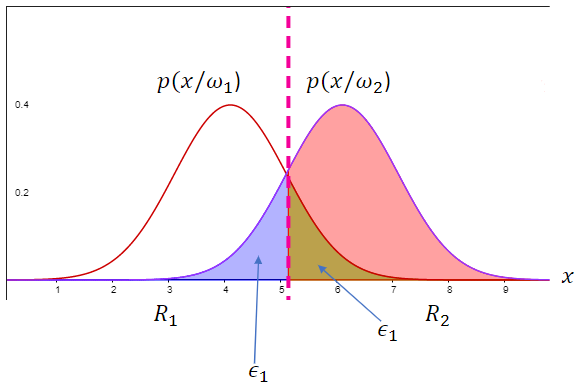
\includegraphics[width=0.9\textwidth]{prob_error.png}}}
		\caption{Probability of Error}
		\label{prob_error}
	\end{figure}
	
	\begin{equation*}
		P_e = P(x \in R_2 | \omega_1)P(\omega_1) + P(\omega_2)P(x \in R_1 | \omega_2)
	\end{equation*}
	
	\begin{equation*}
		= P(\omega_1)\int_{R_2}{p(x|\omega_1)dx} + P(\omega_2)\int_{R_1}{p(x|\omega_2)dx}
	\end{equation*}
	
	\begin{equation*}
		\text{But}\ \int_{R_1}p(x|\omega_2)dx + \int_{R_2}p(x|\omega_2)dx = 1
	\end{equation*}
	
	\begin{equation*}
		\therefore P_e = P(\omega_1)\underbrace{\int_{R_2}p(x|\omega_1)dx}_{\varepsilon_1} + P(\omega_2)\underbrace{\left\{1 - \int_{R_2}p(x|\omega_2)dx\right\}}_{\varepsilon_2}
	\end{equation*}
	
	\begin{equation*}
		= P(\omega_2) + \int_{R_2}\underbrace{\left[P(\omega_1)p(x|\omega_1) - P(\omega_2)p(x|\omega_2)\right]}_{\text{Include}\ x\ \text{in}\ R_2\ \text{if negative}}dx
	\end{equation*}
	
	\begin{equation*}
		P(\omega_1)p(x|\omega_1) \decisionbound P(\omega_2)p(x|\omega_2)
	\end{equation*}
\end{document}